\chapter{The importance of parameter values in the clustering output}

\section{Monocle and Seurat}
As stated in the previous chapter, the PhenoGraph pipeline was widely adopted in the task of processing biological data, due to its efficiency and quality of results. The pipeline was incorporated and implemented in various programming languages.

The most frequently used R packages that perform single-cell data processing are Seurat (currently on the third version) \cite{Hao2021} and Monocle (currently at the third version) \cite{Cao2019}. Both packages use the PhenoGraph method for the cell clustering. The goal of this chapter is to evaluate the output of the two packages and compare the results side by side.

\section{Data used for experiments}
To perform this comparison, we used the Cuomo data \cite{Cuomo2020}, an in-vitro SMART-seq dataset of human endoderm differentiation. The dataset contains 1880 cells extracted from six donors (hayt, naah, vils, pahc, melw and qunz) at four different timepoints. The cells are in expressed in approximately 30 000 genes. The dataset was preprocessed by removing the cells that are expressed in less than 200 features and the genes that are expressed in less than three cells. MT (mitochondrial) and RP (ribosomal protein) genes were also excluded from the feature set.

The purpose of this thesis is to analyze the clustering pipeline, therefore the preprocessing parameters (normalization and scaling) are done in the same manner for both packages.

\section{Algorithms used in the pipeline}
In chapter one we presented the steps that are involved in the PhenoGraph pipeline, namely the dimensionality reduction, the graph construction and the community detection. Each step can be performed by a varying number of algorithms. Therefore, in order to compare the two R packages, we must identify the algorithms that they are using in the clustering pipeline (see Table \ref{tab:s4-m3-methods}).

For the dimensionality reduction, both packages allow the usage of either linear methods (PCA) or non-linear ones (UMAP and tSNE). The developers of the both packages recommend performing the PCA reduction on the raw data, followed by tSNE or UMAP. The graph construction is performed using the kNN based method. For the community detection, Monocle uses the Louvain and Leiden alogrithms, whereas Seurat can cluster the cells using Louvain with multi-level refinement and SLM, too.

We note that all the algorithms involved in the clustering pipeline contain at least one stochastic component, therefore 

\begin{table}[]
    \begin{tabular}{|l|l|l|l|}
        \hline
                         & \textbf{Dim reduction}    & \textbf{Graph construction} & \textbf{Graph clustering} \\ \hline
        \textbf{Seurat}  & \begin{tabular}[c]{@{}l@{}}PCA followed\\ by tSNE or UMAP\end{tabular} & \begin{tabular}[c]{@{}l@{}}kNN based\\ support for SNN\end{tabular}   & \begin{tabular}[c]{@{}l@{}}Louvain, Louvain refined,\\ SLM, Leiden\end{tabular} \\ \hline
        \textbf{Monocle} & \begin{tabular}[c]{@{}l@{}}PCA followed\\ by tSNE or UMAP\end{tabular} & \begin{tabular}[c]{@{}l@{}}kNN based\\ support for SNN\end{tabular}   & Louvain, Leiden           \\ \hline
    \end{tabular}
    \caption{\label{tab:s4-m3-methods}The algorithms used by Monocle and Seurat inside the Phenograph pipeline}
\end{table}

\section{Comparing the results}

\begin{figure}[H]
    \centering
    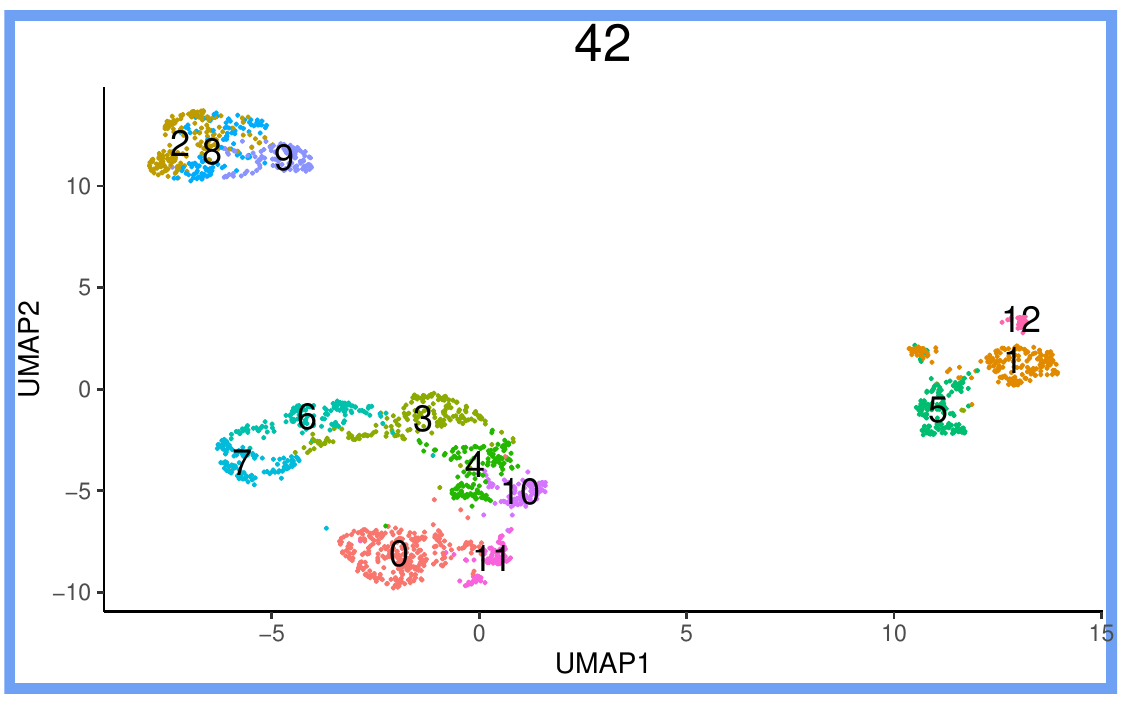
\includegraphics[width=7cm]{2_S1.png}
    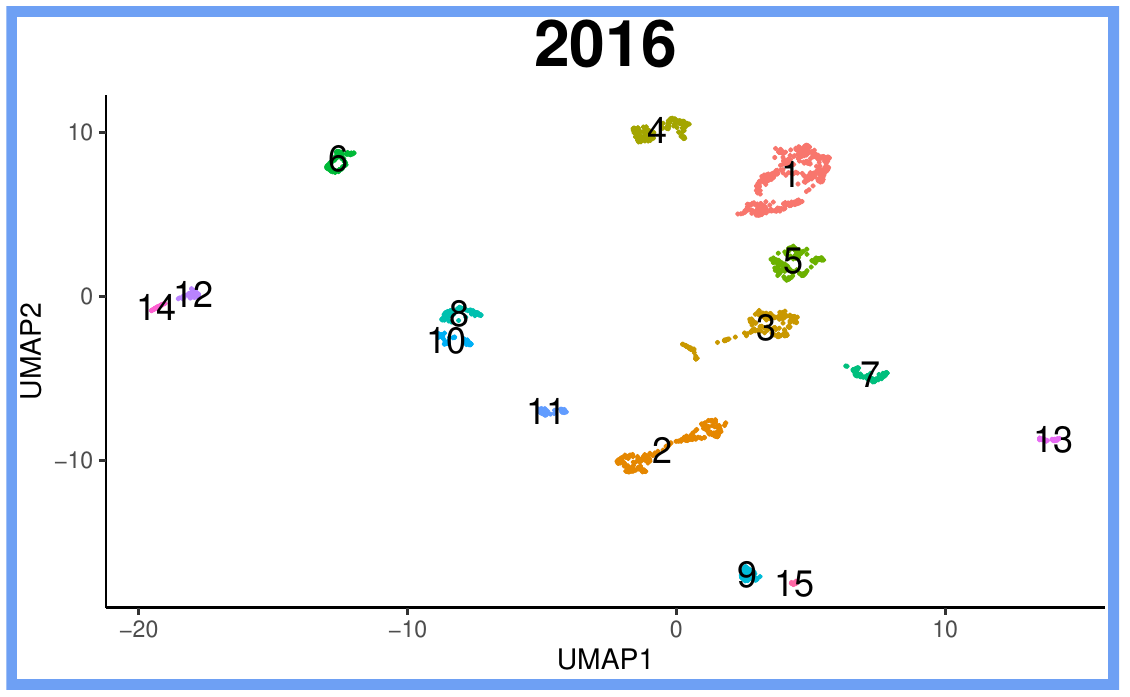
\includegraphics[width=7cm]{2_M1.png}
    \caption{\label{fig:s4-m3-default}Clustering distribution with default parameters for Monocle (right) and Seurat (left). The title indicates the default random seed that is used.}
\end{figure}

If the Cuomo \cite{Cuomo2020} dataset is clustered using the Monocle and Seurat packages with default parameters, significantly different outputs are produced, as it can be observed in Figure \ref{fig:s4-m3-default}. Firstly, there are differences with respect to the dimensionality reduction. The cells are scattered in multiple islands in the Monocle package, whereas Seurat obtains a more compact grouping. Also, the two packages disagree regarding the number of clusters: Seurat outputs 13 clusters, Monocle 15.

The biological interpretation of the data heavily relies on the clusters' structure. Thus, is expected for the discrepancies between the two packages to extend over the marker identification and the biological interpretation. The question we pose is whether the divergence between Monocle and Seurat has technical (such as the implementation of the clustering pipeline) or biological (such as additional pre- or post-processing steps that rely on the sequencing information) causes.

\section{Aligning the results}
We started by analyzing the tehnical differences between the two packages. This involves implementation discrepancies, but also different values of the parameters involved in the clustering process. Our analysis will follow the PhenoGraph pipeline and we will compare the two packages regarding the three steps.

\subsection{Dimensionality reduction}
As stated in the previous sections, both Seurat and Monocle suggest applying PCA on the raw dataset and UMAP or tSNE afterwards. The default choice for non-linear dimensionality reduction is UMAP. As for the implementation, both packages are using the same R packages: \verb|irlba| for PCA (citation) and \verb|uwot| for UMAP (citaton).

The output of the PCA can be affected by parameters such as the number of principal components or the precision of the calculation (the \verb|irlba| package performs an approximate PCA calculation), but the difference between the packages lies in the feature space. Although the data contains up to 30 000 genes, most of them are not appropiate for describing the cells behaviour, as they would introduce more noise than perform any significant separation. Thus, the standard in the processing of the biological data is to choose a relatively small subset of genes that contain discriminative information. By default, Monocle uses all genes, but Seurat performs the PCA only on the genes that have the most variability (citation) (also reffered in literature as highly variable - or HV - genes). Figure \ref{fig:s4-m3-pca} illustrates how the feature set affects the topology. If Seurat uses all genes for PCA, the resulting embedding will contain numerous small islands (see panels S3 and S4). Using only HV genes in Monocle leads to more compact group of cells (see panels M3 and M4).

The UMAP algorithm is signifcantly affected by three parameters:
\begin{itemize}
    \item \textit{the distance metric} that is used in the original space
    \item \textit{the number of neighbours} that is used for building the graph
    \item \textit{the minimum distance} which determines how separated should points be in the low dimensional space. Low values lead to dense groups, while higher values are more preferable for visualisation.
\end{itemize}

Monocle and Seurat agree on the cosine measurement as the distance metric, but the other two parameters have different values in these packages: the minimum distance is 0.3 in Seurat and 0.1 in Monocle, and the number of neighbours is 30 in Seurat and 15 in Monocle. Figures \ref{fig:s4-m3-min-dist} and \ref{fig:s4-m3-n-neigh-umap} highlight the effect of these parameters on the toplogy of the data. Aligning their values for the two packages leads to identical low dimensional representation of the cells, as it can be seen in panels S7 and M8 of the figure \ref{fig:s4-m3-n-neigh-umap}.

\begin{figure}[H]
    \centering
    \makebox[\textwidth][c]{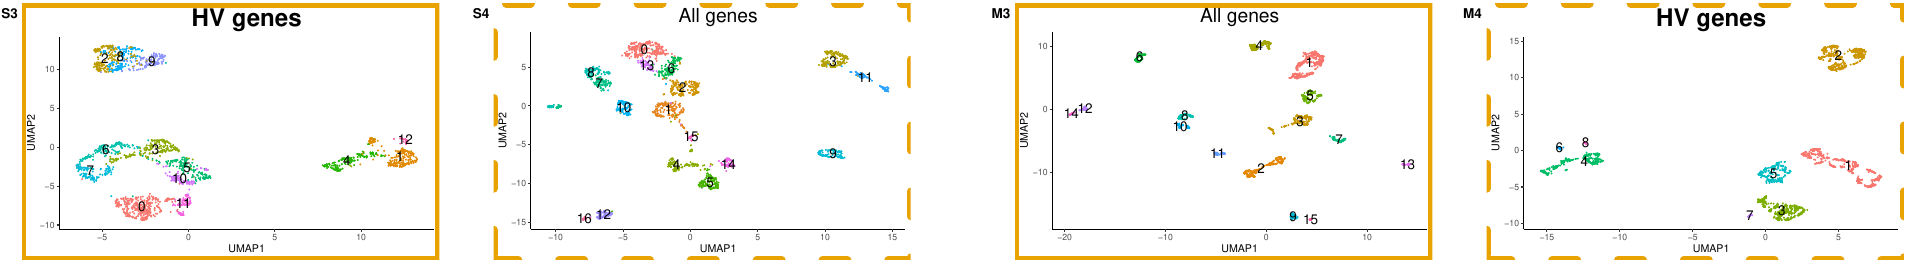
\includegraphics[width=1.2\linewidth]{2_pca_genes.png}}
    \caption{\label{fig:s4-m3-pca}Clustering distribution with default parameters for Monocle (left) and Seurat (right). The title indicates the default random seed that is used.}
\end{figure}


\begin{figure}[H]
    \centering
    \makebox[\textwidth][c]{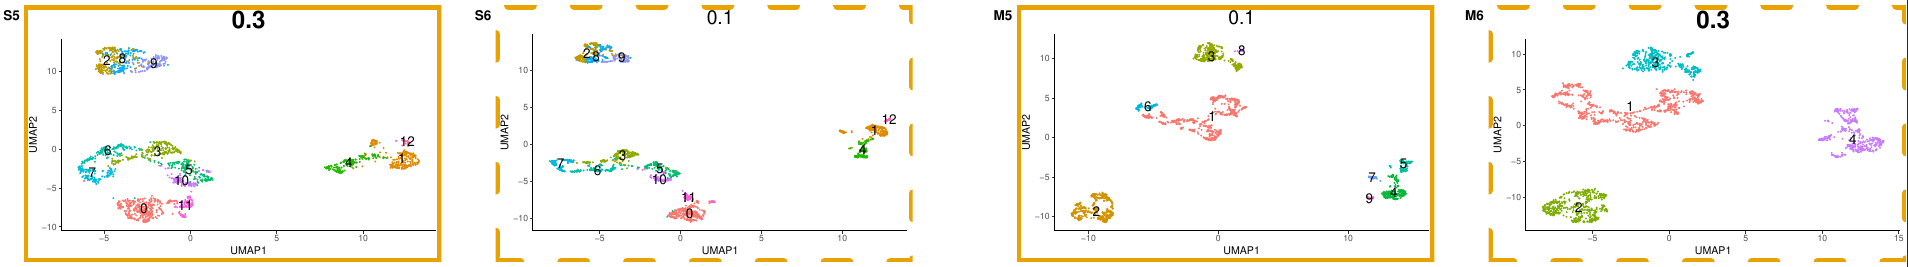
\includegraphics[width=1.2\linewidth]{2_umap_min_dist.png}}
    \caption{\label{fig:s4-m3-min-dist}Clustering distribution with default parameters for Monocle (left) and Seurat (right). The title indicates the default random seed that is used.}
\end{figure}

\begin{figure}[H]
    \centering
    \makebox[\textwidth][c]{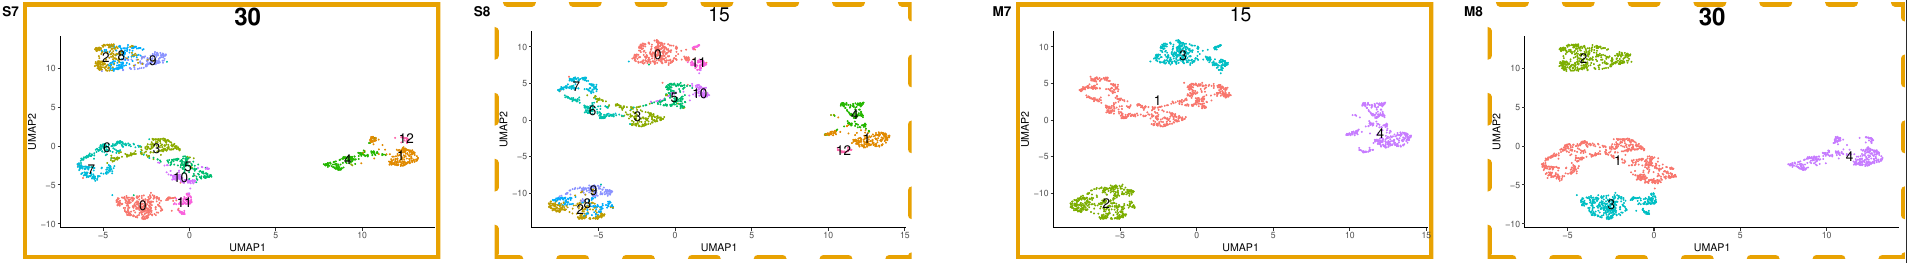
\includegraphics[width=1.2\linewidth]{2_umap_n_neigh.png}}
    \caption{\label{fig:s4-m3-n-neigh-umap}Clustering distribution with default parameters for Monocle (left) and Seurat (right). The title indicates the default random seed that is used.}
\end{figure}

\subsection{Graph construction}
Both packages use the kNN-based method of building the graph based on the reduced space. The output is affected by the embedding that is used as a base for the graph construction, the number of neighbours and the graph type.

\subsection{Graph clustering}










